\documentclass[10pt,letter]{article}
	% basic article document class
	% use percent signs to make comments to yourself -- they will not show up.

\usepackage{amsmath}
\usepackage{amssymb}
	% packages that allow mathematical formatting

\usepackage{graphicx}
	% package that allows you to include graphics

\usepackage{setspace}
	% package that allows you to change spacing

\onehalfspacing
	% text become 1.5 spaced

\usepackage{fullpage}
	% package that specifies normal margins
	
\usepackage[version=3]{mhchem} % Package for chemical equation typesetting
\usepackage{graphicx} % Required for the inclusion of images
\usepackage{natbib} % Required to change bibliography style to APA
\usepackage{amsmath} % Required for some math elements 
\usepackage{booktabs}
\usepackage{floatrow}
	

\begin{document}
	% line of code telling latex that your document is beginning


\title{CS 156 Final Exam}

\author{Christopher Zhen}

\date{Dec 2, 2016}
	% Note: when you omit this command, the current dateis automatically included
 
\maketitle 
	% tells latex to follow your header (e.g., title, author) commands.
	
\section*{Problem 1}

\textbf{(E)} - Since we can find the number of terms by considering the binomial expansion of $(1 + x + y)$. We see that there are 65 terms (not including the $z_0$ term) which is none of the answer choices.

\section*{Problem 2}

\textbf{(D)} - It's possible to have an expected $\bar{g}$ that is not an element of the logistic regression set because if we imagine taking the expected value of $\frac{e^{\mathbf{w}^\textrm{T}\mathbf{x}}}{1+e^{\mathbf{w}^\textrm{T}\mathbf{x}}}$ for different hypotheses $\mathbf{w}^\textrm{T}$, we won't necessarily get something of the same form.

\section*{Problem 3} 

\textbf{(D)} - Overfitting is when our hypothesis is overly complex for the sample data set and as a result doesn't model the true data set. Hence, the difference between $E_{\textrm{in}}$ and $E_{\textrm{out}}$ is a good way to look for potential overfitting, however there can be cases where by random variation a simple hypothesis fits the test set better, but the actual data set worse, and is not a case of overfitting.

\section*{Problem 4}

\textbf{(D)} - Since deterministic noise is the bias, it definitely occurs with stochastic noise and is dependent on both the target function and hypothesis set. Stochastic noise is simply a function of the data set, so it is not a function of the hypothesis set. 

\section*{Problem 5}

\textbf{(A)} - Since we are trying to minimize the error subject to the condition that $\mathbf{w^T \Gamma ^T \Gamma  w} \leq C$ and we know that $\mathbf{w}_{lin}$ already satisfies this condition, then we know that $\mathbf{w}_{reg}$ = $\mathbf{w}_{lin}$.

\section*{Problem 6}

\textbf{(B)} - By introducing soft-order constraints, we are minimizing an error that has an extra term and these augmented errors are minimized in regularization models.

\section*{Problem 7}

\textbf{(D)} - Among the choices the 8 versus all classifier has the lowest $E_{in}$ with an $E_{in}$ of 0.0743.

\begin{figure}[H]
\begin{center}
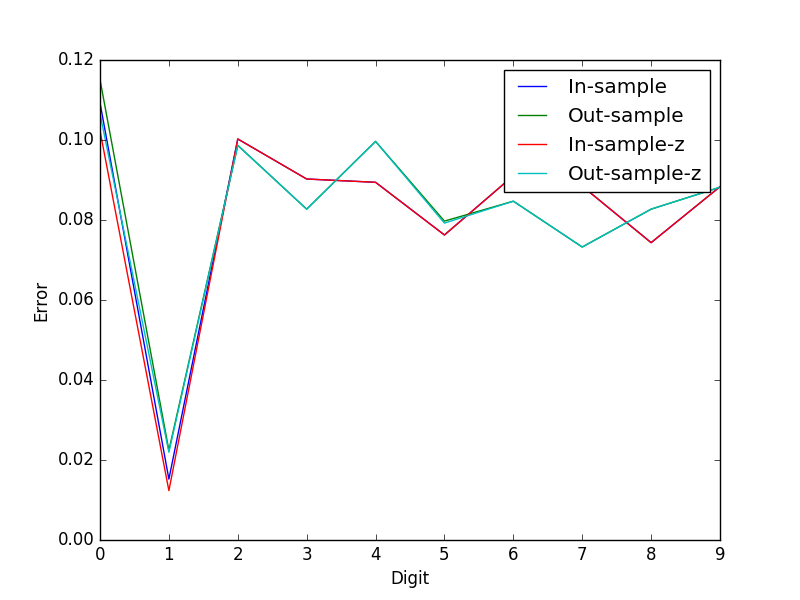
\includegraphics[width=0.75\textwidth]{p7.png}
\caption{Plot of errors for each digit}
\end{center}
\end{figure}

\section*{Problem 8}

\textbf{(B)} - Among the choices, the 1 versus all classifier has the lowest $E_{out}$ with an $E_{out}$ of 0.0219.

\section*{Problem 9}

\textbf{(E)} - The transform makes a slight improvement for a few of the digits. One of which is the digit 5 which has an out of sample improvement from 0.07972 to 0.07922.

\section*{Problem 10}

\textbf{(A)} - Going from $\lambda = 1$ to $\lambda = 0.01$, we get a decrease from 0.00512 to 0.00448 in $E_{in}$ and an increase from 0.0259 to 0.0283 in $E_{out}$. Thus it's possible that there is some overfitting going on since we're decreasing our in-sample error going from $\lambda = 1$ to $\lambda = 0.01$ at the cost of the out-of-sample error.

\section*{Problem 11}

\textbf{(C)} - After performing the transformation, we can see that the data is linearly separable by a vertical line at x = 0.5, so the best choice would be answer choice C.

\section*{Problem 12}

\textbf{(C)} - I couldn't get quadprog to work, so I used the sklearn package (which should give the same results as quadprog). From this I got that there are 5 support vectors. This makes sense because graphically there are 5 points along the boundary between +1 and -1.

\section*{Problem 13}

\textbf{(A)} - Our code shows that the data is almost never not separable using the RBF kernel ($E_out$ is always 0).

\section*{Problem 14}

\textbf{(E)} - Our code gives that 88\% of the time the kernel method gives a lower $E_{out}$. See the following pretty plot for implementation of our Lloyd's algorithm:

\begin{figure}[H]
\begin{center}
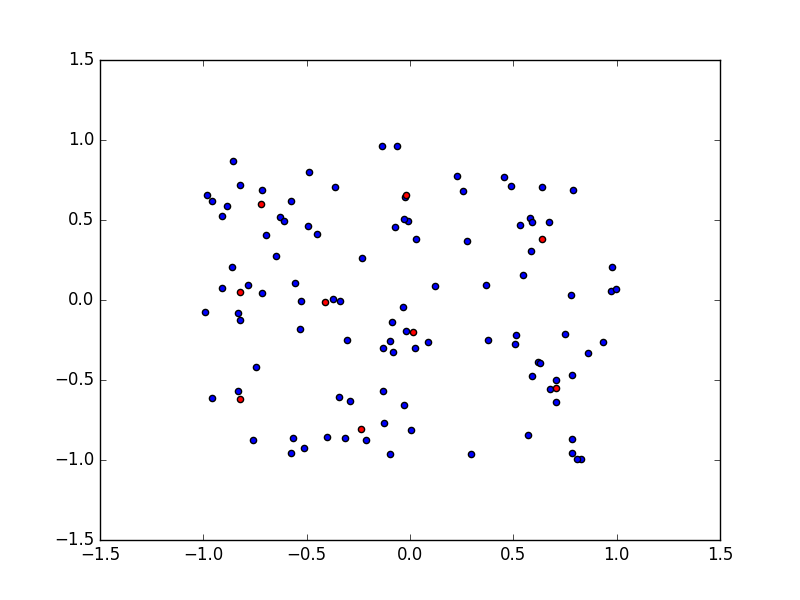
\includegraphics[width=0.8\textwidth]{lloyds_alg.png}
\caption{Result of using Lloyd's algorithm to assign centers (red points) to a data set}
\end{center}
\end{figure}

\section*{Problem 15}

\textbf{(D)} - Our code gives that 78\% of the time the kernel method gives a lower $E_{out}$. It makes sense for this value to be lower than in 14 because the $K = 12$ regular RBF should be more accurate than the one with 9 centers.

\section*{Problem 16}

\textbf{(D)} - Our code gives us that in 100 trials, answer D happens 34 times with the next most frequent answer being A which only happens 9 times.

\section*{Problem 17}

\textbf{(C)} - After running the code for 1000 trials, answer choice C happens 313 times while the next closest answer (D) happens 188 times.

\section*{Problem 18}

\textbf{(A)} - After running the code for 1000 trials, I found that regular RBF achieves $E_in = 0$ less than 0.04 of the time.

\section*{Problem 19}

\textbf{(B)} - The Bayesian prior becomes an increasing function from 0 to 1 because given our new data, we now know that h = 0 is impossible and h = 1 is most likely. It's a linearly increasing function because there's not enough information to deduce a different distribution.

\section*{Problem 20}

\textbf{(C)} - Since g(x) is the average hypothesis, it makes sense that the error of g(x) is lower than at least one of the errors of g$_{1}$ and g$_2$. Thus it is not necessarily better than both errors (for example if g$_1$ is a very good hypothesis and g$_2$ is really bad, then the error of g is in between the two). We can also envision a situation where the error is better than both errors of g$_1$ and g$_2$. This eliminates all choices but C and E. We can further see that the error can't be worse than the average of the other two errors because that's the case where neither hypothesis helps correct the other, so at worst we'll be as good as the average of the two.

\end{document}
	% line of code telling latex that your document is ending. If you leave this out, you'll get an error
